%
% File for Section 1.3
%
%
% The following is only needed for out of sequence paragraphs
% enable only if required
\setcounter{section}{2}
%
\section{Ενθυλάκωση}
\begin{inthebox}
\emph{Τι σημαίνει ενθυλάκωση;} Προέρχεται από το ρήμα ενθυλακώνω που σημαίνει ``βάζω σε θύλακα (τσέπη)''. Εδώ χρησιμοποιείται για να εξηγήσει πως κάθε επίπεδο προσθέτει τις δικές του πληροφορίες (με τη μορφή επικεφαλίδας) στα δεδομένα που έχει λάβει από το πιο πάνω επίπεδο.\\
\end{inthebox}

\begin{figure}[!ht]
  \centering
  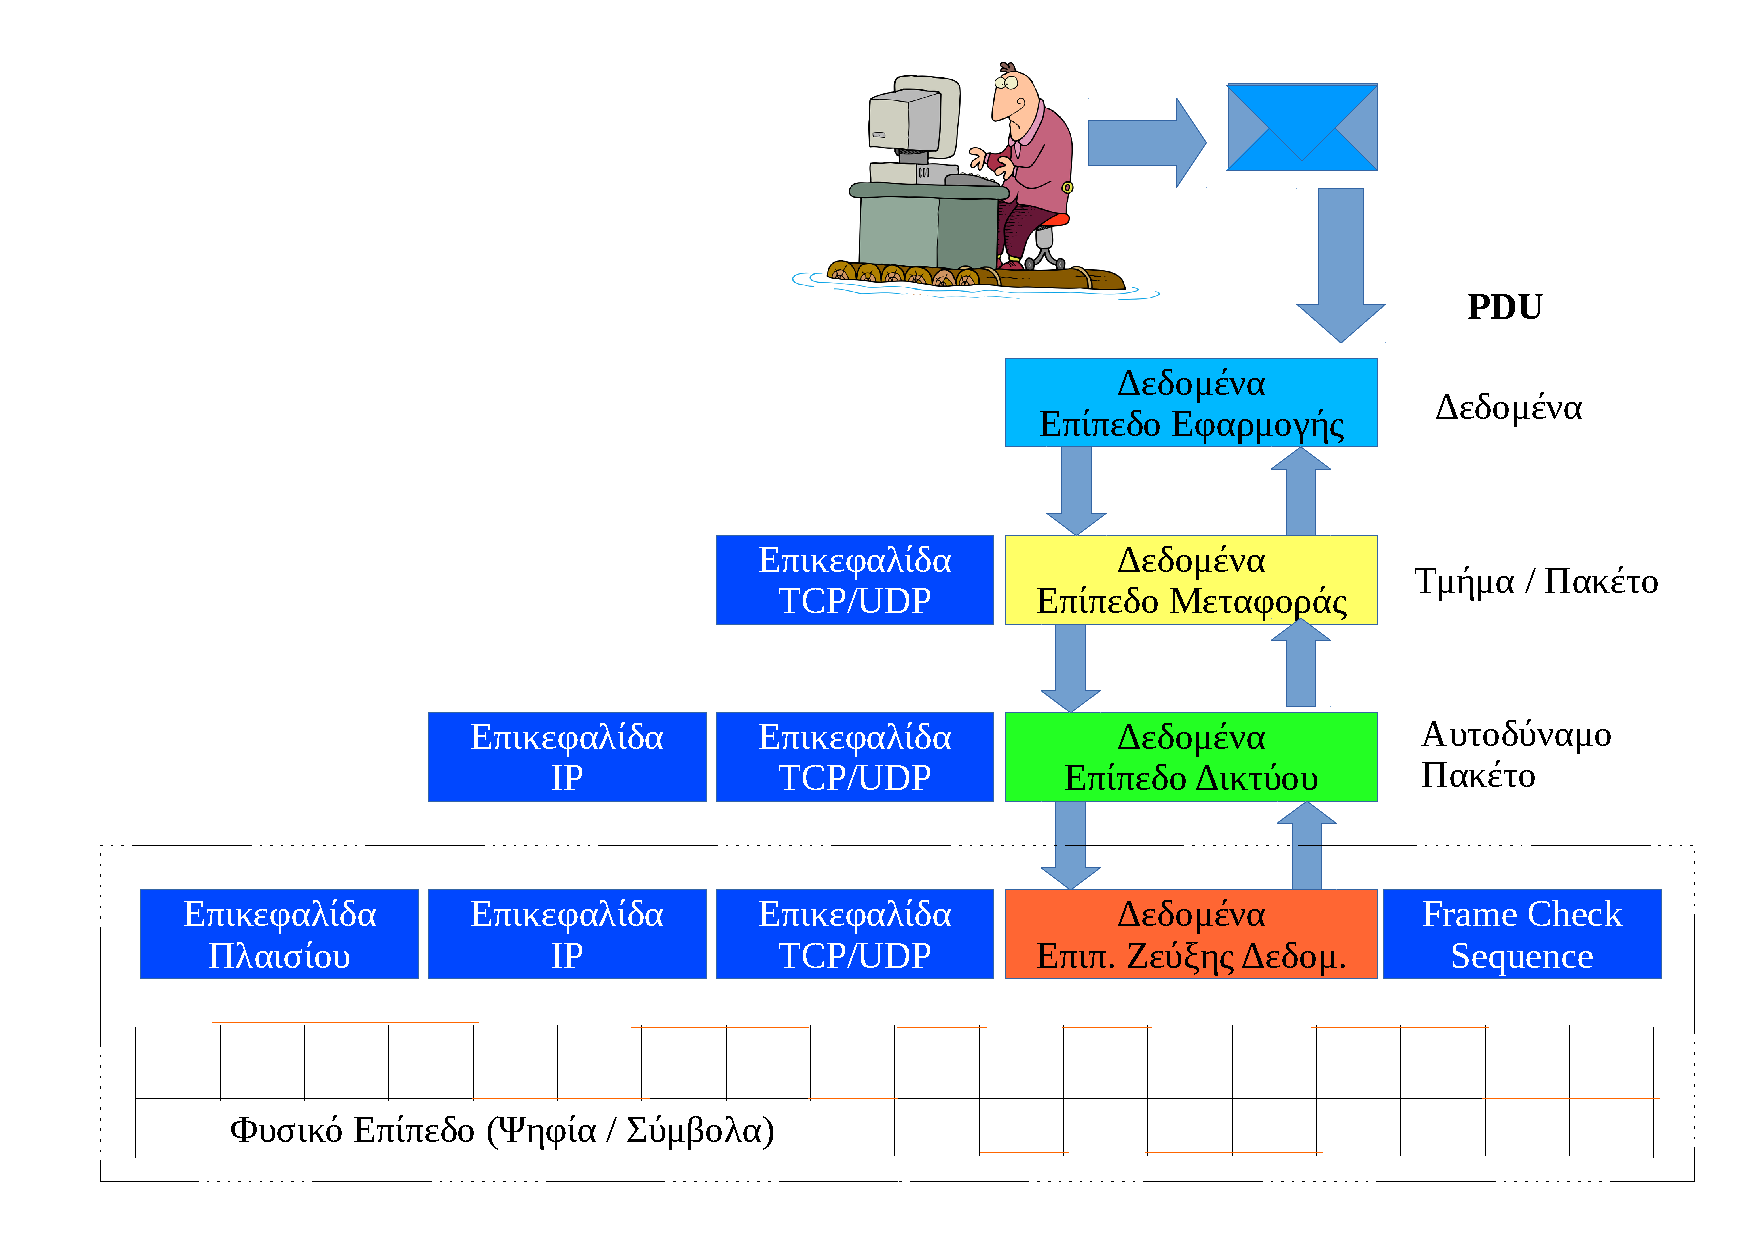
\includegraphics[width=1.00\textwidth]{images/chapter1/1-3}
  \caption {\textsl{Ενθυλάκωση}}
  \label{1-3}
\end{figure}

Όπως έχουμε ήδη εξηγήσει στο πρότυπο OSI, σε μια επικοινωνία μεταξύ των κόμβων Α και Β, το κάθε επίπεδο του Α φαίνεται να επικοινωνεί απευθείας με το αντίστοιχο (ομότιμο) επίπεδο του Β. Έτσι για παράδειγμα το επίπεδο εφαρμογής του Α φαίνεται να επικοινωνεί απευθείας με το επίπεδο εφαρμογής του Β. Θυμηθείτε την εργαστηριακή επίδειξη του πρωτοκόλλου SMTP, που είναι ένα από τα κλασικά πρωτόκολλα στο επίπεδο εφαρμογής. Καθώς το επίπεδο εφαρμογής είναι το υψηλότερο, οι εντολές που χρησιμοποιεί είναι αρκετά κατανοητές από τον άνθρωπο και είδαμε ότι μπορούμε να τις δώσουμε από το τερματικό. Κατά τη διάρκεια της επικοινωνίας μας με τον SMTP δίναμε μόνο εντολές που είχαν να κάνουν με την αποστολή ενός μηνύματος ταχυδρομείου σε μια αντίστοιχη διεύθυνση ηλεκτρονικού ταχυδρομείου: δεν ασχοληθήκαμε καθόλου με λεπτομέρειες όπως τη διεύθυνση IP του εξυπηρετητή, ή τον τρόπο αποστολής των πακέτων από τον ένα υπολογιστή στο άλλο. Όλα αυτά δεν απασχολούν το πρωτόκολλο εφαρμογής γιατί εξυπηρετούνται από πρωτόκολλα σε χαμηλότερα επίπεδα. Αν και η επίδειξη έγινε ανάμεσα σε δύο μηχανήματα του εργαστηρίου, ακόμα και αν γινόταν μεταξύ ενός τοπικού και ενός απομακρυσμένου μηχανήματος, δεν θα άλλαζε σε κάτι όσο αφορά εμάς. Το πρωτόκολλο εφαρμογής της μιας μεριάς φαίνεται να επικοινωνεί απευθείας με το πρωτόκολλο εφαρμογής της άλλης.

Ωστόσο η πραγματικότητα είναι διαφορετική: αν και το πρωτόκολλο εφαρμογής νομίζει το ίδιο ότι μιλάει απευθείας με το ομότιμο του στην άλλη πλευρά, στην πραγματικότητα τα δεδομένα που παράγει προωθούνται στα παρακάτω, κατώτερα επίπεδα. Σε κάθε επίπεδο προστίθεται στα δεδομένα του προηγούμενου μια νέα επικεφαλίδα.

\begin{inthebox}
\emph{Τι είναι η επικεφαλίδα;} Φανταστείτε ότι θέλετε να στείλετε ένα γράμμα (κανονικό, όχι email). Τα περιεχόμενα του γράμματος είναι τα δεδομένα σας. Το βάζετε σε ένα φάκελο. Αυτός είναι ο θύλακας (μόλις κάνατε μια ενθυλάκωση!) Πάνω στο φάκελο γράφετε τη διεύθυνση σας και τη διεύθυνση παραλήπτη. Αυτή είναι η επικεφαλίδα του πρωτοκόλλου εφαρμογής. Το ρίχνετε στο ταχυδρομείο και από κει και πέρα δεν ξέρετε με ποιο τρόπο θα πάει. Όσο αφορά εσάς, το γράμμα σας απλά θα πάει στο ίδιο επίπεδο στην άλλη μεριά (τον παραλήπτη).

Έστω ότι το γράμμα σας πηγαίνει από Χανιά στην Θεσσαλονίκη. Στο ταχυδρομείο, όλα τα γράμματα που κατευθύνονται προς Θεσσαλονίκη θα μπουν σε ένα μεγάλο σάκο με ένδειξη ``Θεσσαλονίκη''. Το ταχυδρομείο έκανε ακόμα μια ενθυλάκωση: πήρε το γράμμα σας και το περιέκλεισε σε ένα άλλο ``φάκελο'' προσθέτοντας τη δική του επικεφαλίδα. Ο σάκος θα πάει στην αεροπορική εταιρεία όπου θα μπει σε ένα κοντέινερ μαζί με άλλα δέματα και αποσκευές και θα κολληθεί ένα bar code που αντιστοιχεί στο αεροδρόμιο Θεσσαλονίκης. Ακόμα μια ενθυλάκωση.

Καθώς φαντάζεστε, στην πλευρά του παραλήπτη ακολουθείται η αντίστροφη διαδικασία, όπου διαδοχικά αφαιρούνται οι επικεφαλίδες και ακολουθείται μια διαδικασία παράδοσης μέχρι τον τελικό παραλήπτη. Τίποτα όμως από αυτή τη διαδικασία δεν είναι γνωστή (και ούτε ενδιαφέρει) το επίπεδο εφαρμογής.\\
\end{inthebox}

Στο TCP/IP έχουμε ακριβώς την ίδια διαδικασία, καθώς και αυτό είναι ένα διαστρωματωμένο πρωτόκολλο: το κάθε επίπεδο δημιουργεί μια επικεφαλίδα που περιέχει πληροφορίες απαραίτητες για το αντίστοιχο επίπεδο της άλλης μεριάς. Π.χ. σε ένα μήνυμα ηλεκτρονικού ταχυδρομείου, το επίπεδο εφαρμογής θα βάλει τις διευθύνσεις email παραλήπτη και αποστολέα. Στην πραγματικότητα βέβαια το μήνυμα δεν θα πάει απευθείας αλλά θα περάσει διαδοχικά από τα επίπεδα μεταφοράς, δικτύου και διεπαφής δικτύου. Σε καθένα από αυτά τα επίπεδα θα προστεθεί η αντίστοιχη επικεφαλίδα που είναι απαραίτητη ώστο το επίπεδο να επικοινωνεί με το αντίστοιχο της άλλης μεριάς. Η επικεφαλίδα περιέχει ουσιαστικά πληροφορίες ελέγχου για να μπορεί να γίνει σωστά η ανασύνθεση των δεδομένων στην άλλη μεριά (τα δεδομένα μπορεί να μεταφέρονται σε μικρά κομμάτια). Σε κάποια επίπεδα (όπως στο 2ο του OSI) προστίθενται και πληροφορίες στο τέλος που έχουν να κάνουν με διόρθωση και έλεγχο σφαλμάτων μετάδοσης στο φυσικό μέσο. Η προσθήκη σαν περίβλημα των πληροφοριών ελέγχου με τη μορφή της επικεφαλίδας είναι η ενθυλάκωση.

Σε κάθε επίπεδο στο TCP/IP η μορφή των δεδομένων που προκύπτει μετά την ενθυλάκωση έχει συγκεκριμένη ονομασία (αν και πολλές φορές παρασυρόμαστε και λέμε παντού τη λέξη ``πακέτο''). Η μορφή γενικά ονομάζεται \textbf{PDU, Protocol Data Unit} ή \textbf{Βασική Μονάδα Πληροφορίας Πρωτοκόλλου}. Στο TCP/IP έχουμε τα παρακάτω PDU:

\begin{itemize}
\item \textbf{Επίπεδο Εφαρμογής:} \emph{Δεδομένα}
\item \textbf{Επίπεδο Μεταφοράς:} \emph{Τμήμα (Segment) στο TCP ή Πακέτο (Packet) στο UDP}
\item \textbf{Επίπεδο Δικτύου:} \emph{Αυτοδύναμο Πακέτο (Datagram)}
\item \textbf{Επίπεδο Διεπαφής Δικτύου:} \emph{Πλαίσιο (Frame) (για δίκτυα Ethernet, στο υποεπίπεδο ζεύξης δεδομένων} και \emph{Δυαδικά ψηφία - σύμβολα (Bits / Symbols) στο φυσικό υποεπίπεδο}
\end{itemize}

Έχουμε ήδη αναφέρει ότι το TCP/IP δεν ορίζει ακριβώς τι γίνεται στο κατώτερο επίπεδο. Η μόνη απαίτηση εδώ είναι να μπορεί να μεταφέρει με κάποιο τρόπο τα αυτοδύναμα πακέτα IP που δημιουργούνται, στο φυσικό μέσο. Ένα αυτοδύναμο πακέτο IP από το επίπεδο διαδικτύου τοποθετείται μέσα (ενθυλακώνεται) σε ένα πλαίσιο (frame) που δημιουργείται στο επίπεδο ζεύξης δεδομένων. Το πλαίσιο έχει την δική του επικεφαλίδα καθώς και κάποιες πληροφορίες ελέγχου στο τέλος (Frame Check Sequence, ακολουθία ελέγχου πλαισίου ή FCS). Με απλά λόγια, ένα ``πακέτο'' ανώτερου επιπέδου τοποθετείται εξ'ολοκλήρου (ενθυλακώνεται) μέσα σε ένα ``πακέτο'' του αμέσως κατώτερου επιπέδου. Η διαδικασία αυτή γίνεται τυπικά από το πρόγραμμα οδήγησης (driver) της κάρτας δικτύου.

Οι πληροφορίες ελέγχου που προστίθενται κατά τη διαδικασία ελέγχου είναι κυρίως \emph{διευθύνσεις, χαρακτήρες ελέγχου σφαλμάτων ή άλλοι χαρακτήρες ελέγχου και συγχρονισμού}. Στο φυσικό πλέον επίπεδο τα μηδέν και ένα (δυαδικά ψηφία) που απαρτίζουν το πλαίσιο μετατρέπονται σε κατάλληλα ηλεκτρικά σήματα για να μεταδοθούν μέσα από το φυσικό μέσο. Η διαδικασία αυτή γίνεται από το υλικό (hardware) της κάρτας δικτύου. Στη λήψη δεδομένων γίνεται η ακριβώς αντίστροφη διαδικασία, με τα δεδομένα να κινούνται προς τα ανώτερα επίπεδα όπου αφαιρούνται διαδοχικά οι επικεφαλίδες, μέχρι να φτάσουμε στο επίπεδο εφαρμογής.